\chapter{Results, Demonstration and Discussion}
\label{ch:results}

\section{Implemented Features}
All objectives O1--O7 are implemented: role-based portals over 44 routes; the four-model synthetic
ensemble with per-model votes and explanations; the patient vault with scoped, expiring, use-limited QR
passes and an audit log; optional de-identified Gemini narratives; the MIMIC-IV Demo task with grouped
cross-validation; loopback-only research serving with verified artifacts, a model-analytics page, a
what-if estimator and a stay-level research triage page; and production hardening.

\section{Screenshots and Demonstration Evidence}
The screenshots below were captured on 26~October~2026 from the running application with an automated
browser (Microsoft Edge driven by Playwright). Synthetic pages use a copy of the synthetic demo database;
research pages show aggregate results only (the research triage page is cropped to its summary cards).

\begin{figure}[!htbp]
\centering
\begin{minipage}{0.495\linewidth}\centering
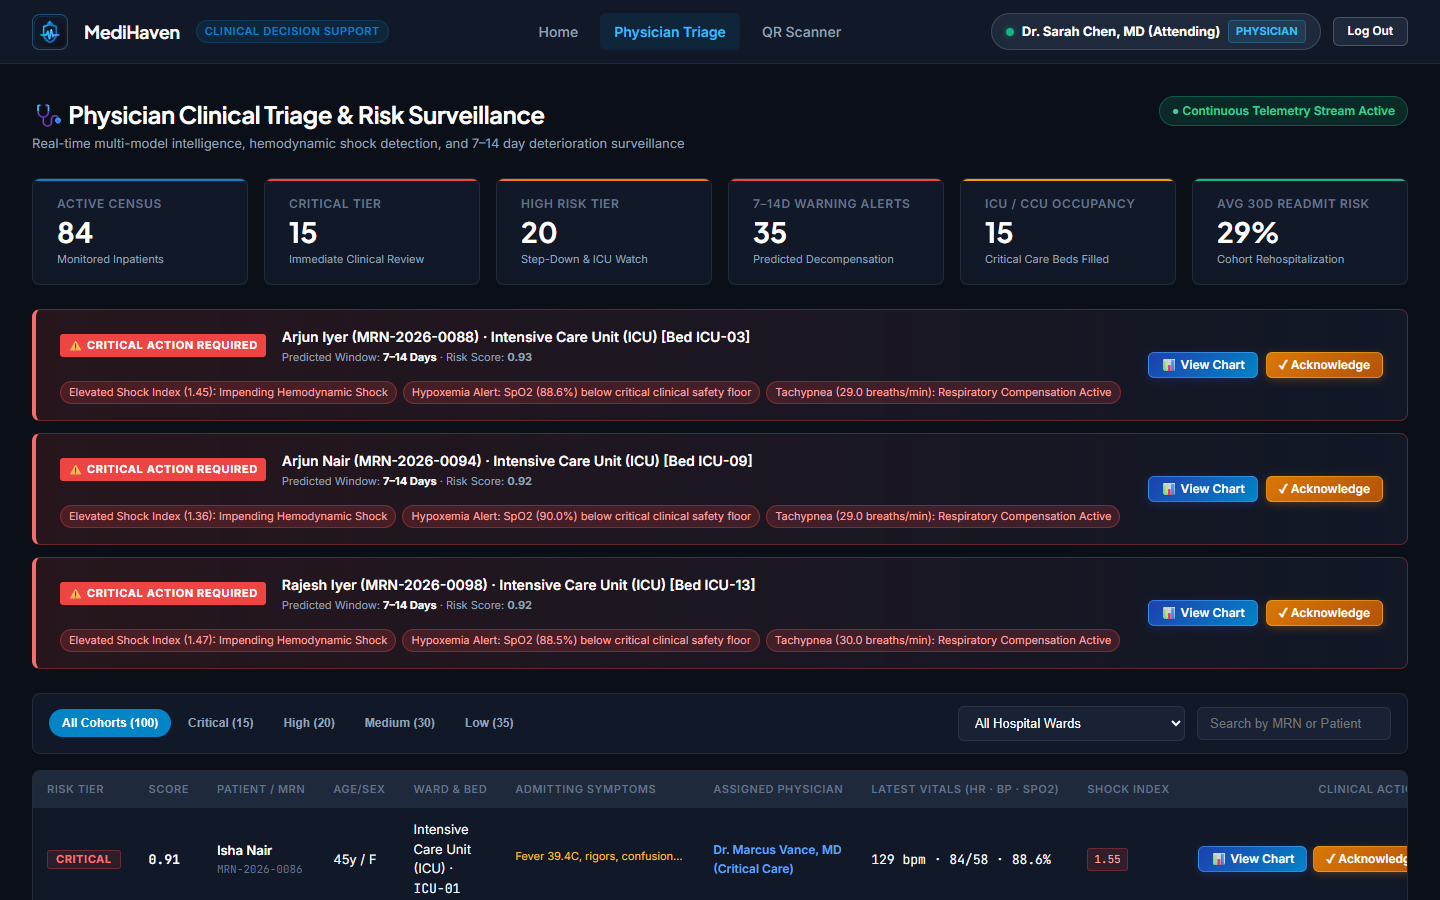
\includegraphics[width=\linewidth]{figures/screenshots/03_triage_dashboard.png}\\[-1pt]
{\footnotesize (a) Triage dashboard: KPIs, alert feed, roster}
\end{minipage}\hfill
\begin{minipage}{0.495\linewidth}\centering
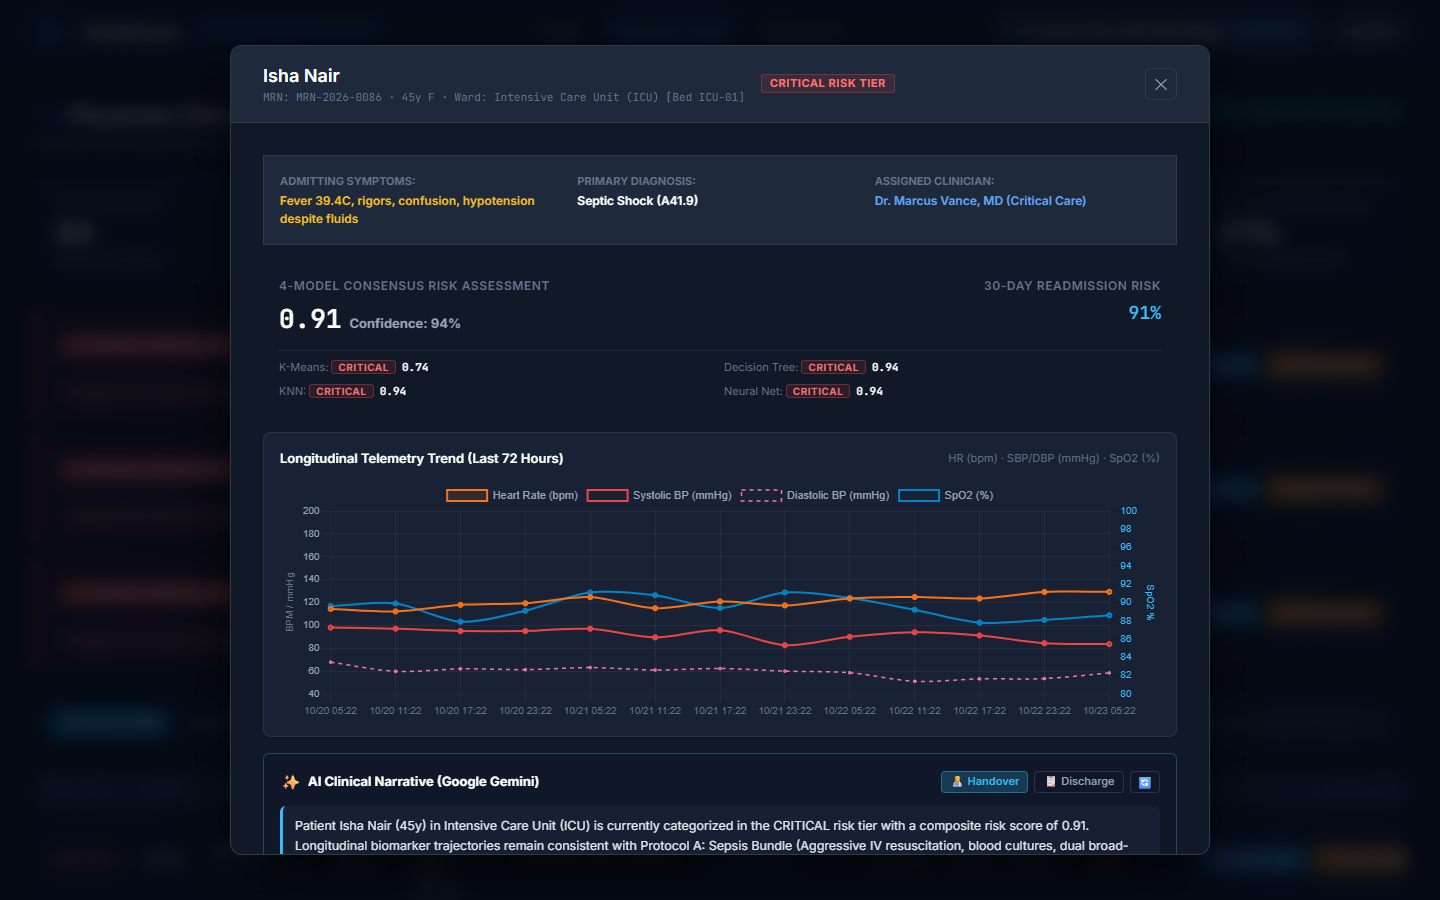
\includegraphics[width=\linewidth]{figures/screenshots/04_patient_chart_drawer.png}\\[-1pt]
{\footnotesize (b) Patient chart: 4 model votes and 72-h vitals}
\end{minipage}
\caption{Physician portal on the synthetic cohort}
\label{fig:ss-triage}
\end{figure}

\begin{figure}[!htbp]
\centering
\begin{minipage}{0.495\linewidth}\centering
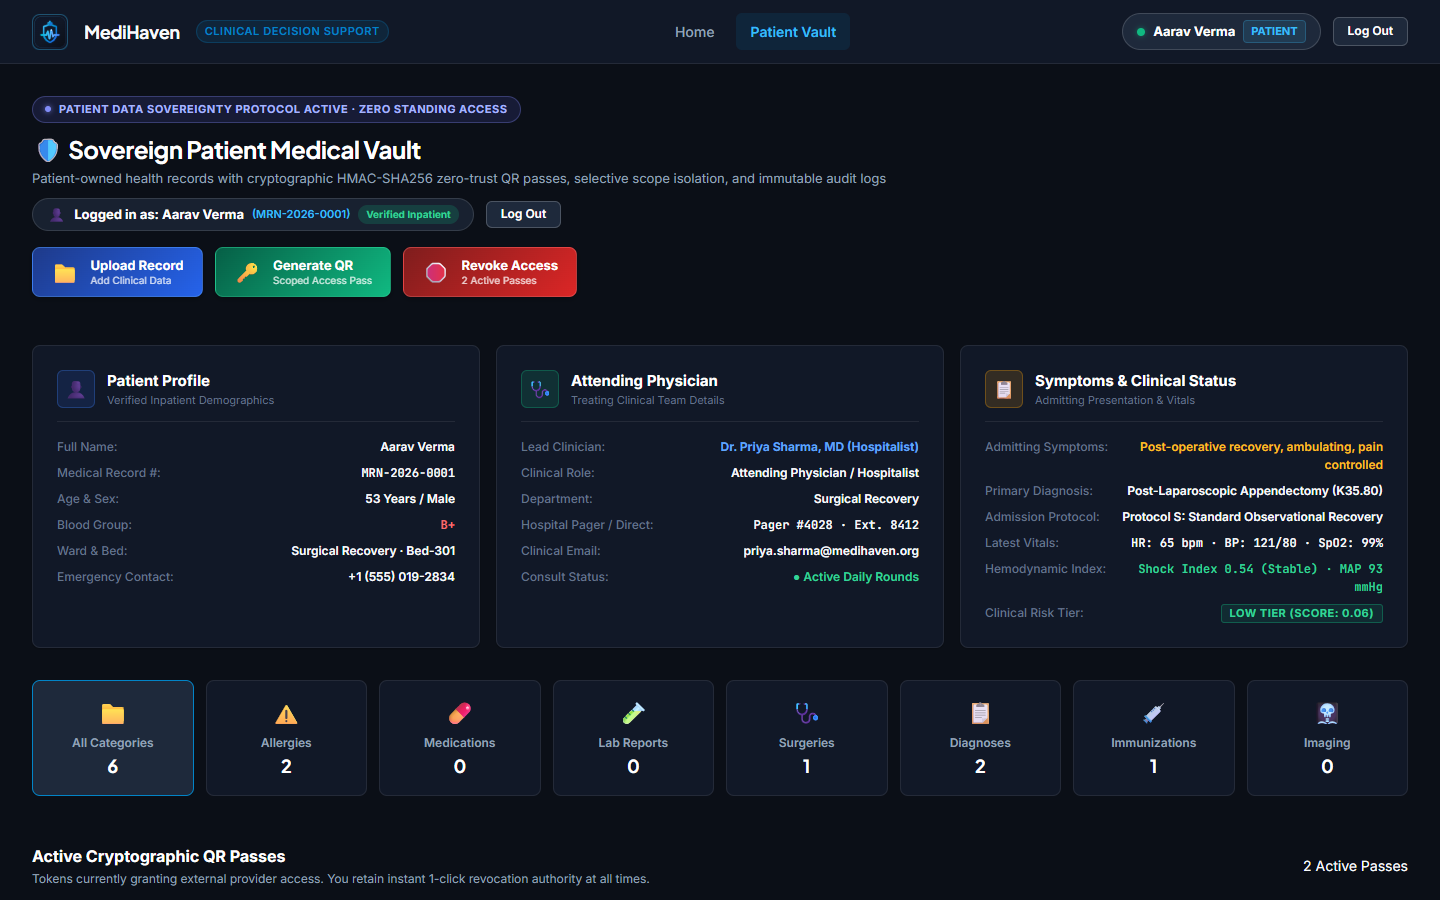
\includegraphics[width=\linewidth]{figures/screenshots/06_patient_vault.png}\\[-1pt]
{\footnotesize (a) Patient vault}
\end{minipage}\hfill
\begin{minipage}{0.495\linewidth}\centering
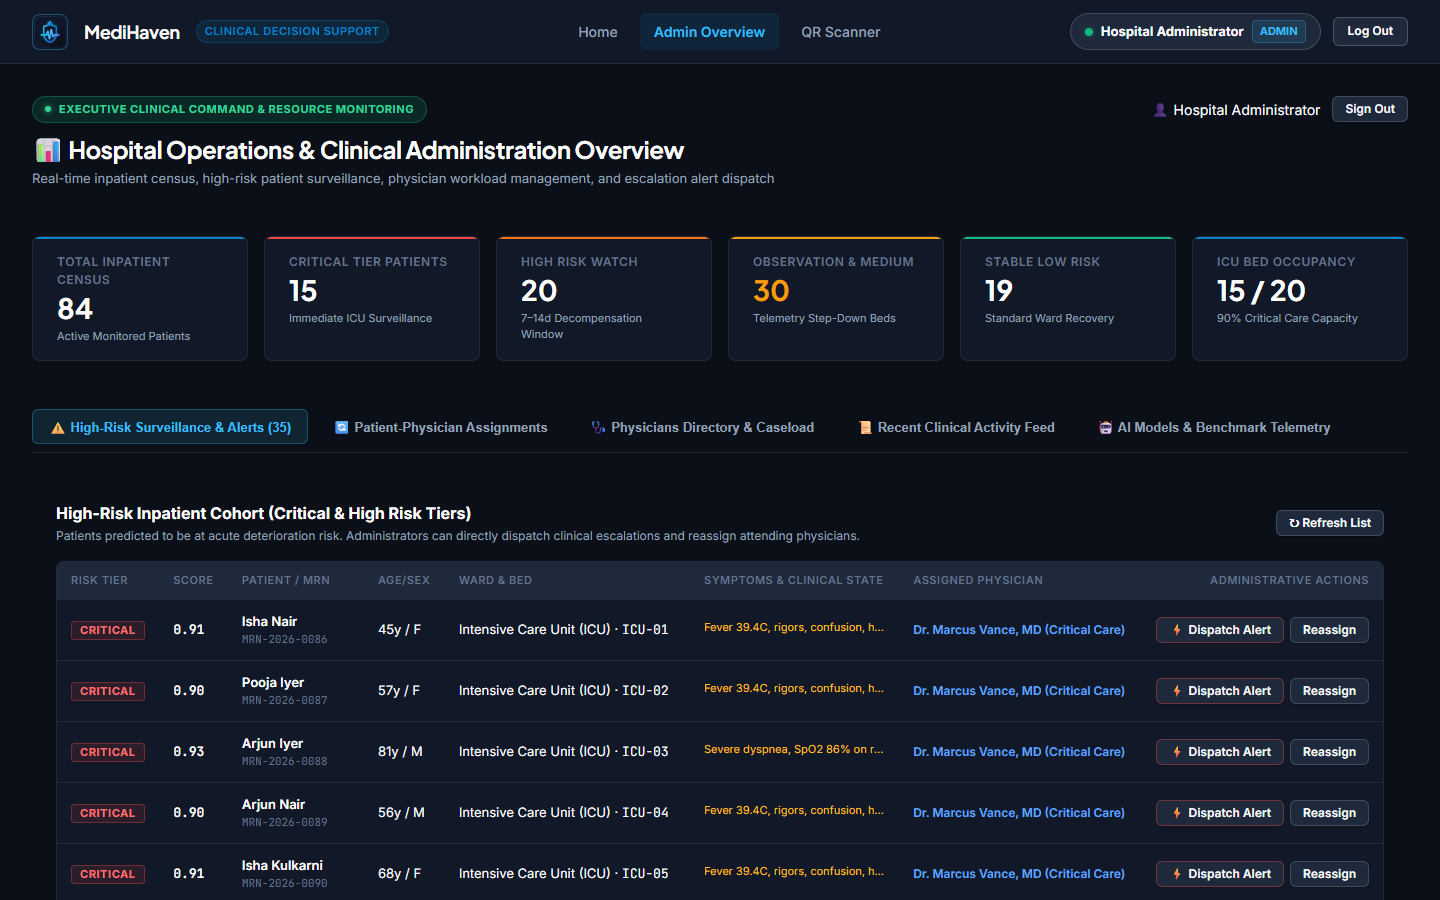
\includegraphics[width=\linewidth]{figures/screenshots/07_admin_overview.png}\\[-1pt]
{\footnotesize (b) Administrator overview}
\end{minipage}\\[6pt]
\begin{minipage}{0.55\linewidth}\centering
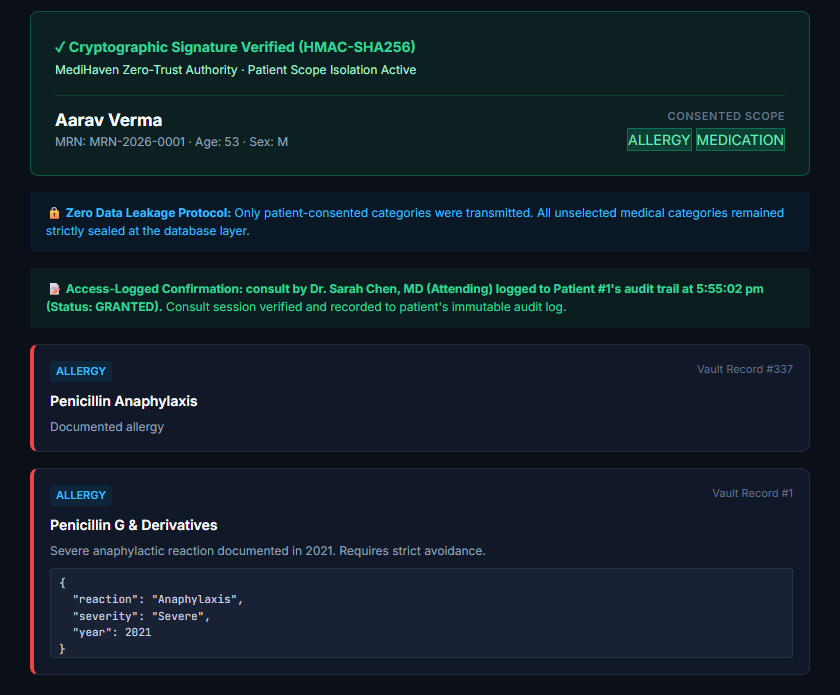
\includegraphics[width=\linewidth]{figures/screenshots/05_qr_scanner_result.png}\\[-1pt]
{\footnotesize (c) QR scanner result: only the consented categories, access logged under the signed-in clinician}
\end{minipage}
\caption{Patient, administrator and scanner portals (synthetic data)}
\label{fig:ss-portals}
\end{figure}

\begin{figure}[!htbp]
\centering
\begin{minipage}{0.495\linewidth}\centering
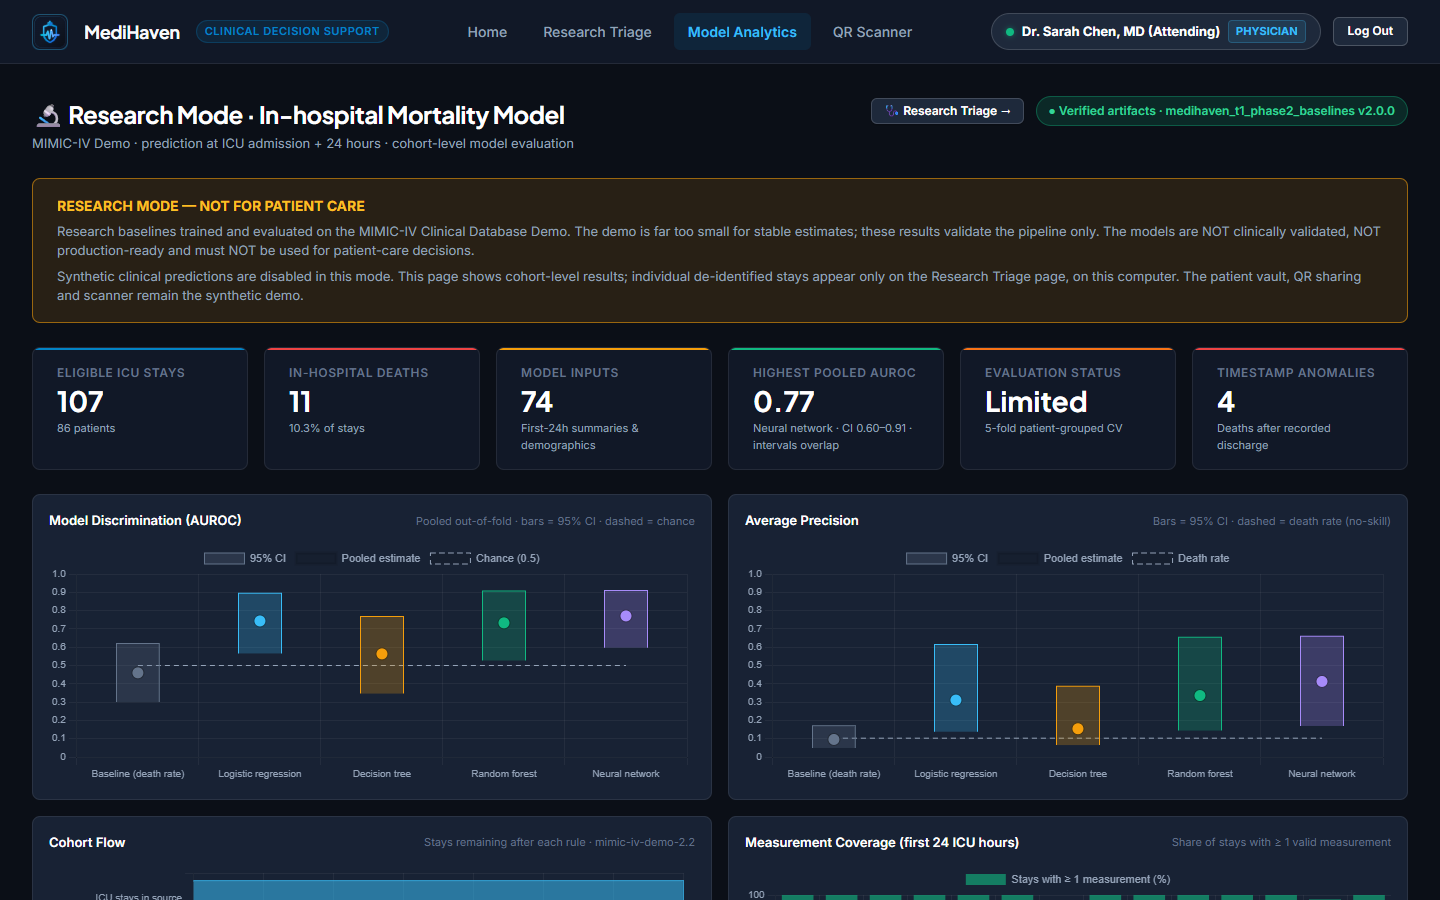
\includegraphics[width=\linewidth]{figures/screenshots/08_research_analytics_top.png}\\[-1pt]
{\footnotesize (a) Model analytics (cohort level)}
\end{minipage}\hfill
\begin{minipage}{0.495\linewidth}\centering
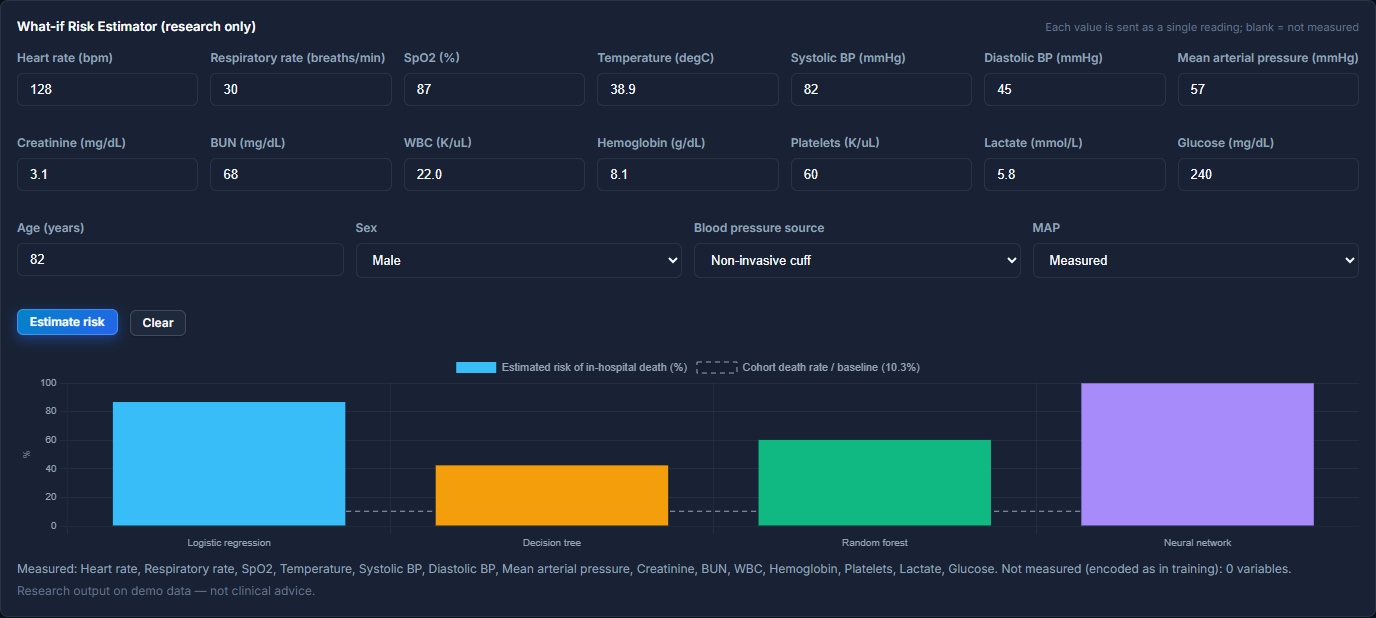
\includegraphics[width=\linewidth]{figures/screenshots/09_research_whatif.png}\\[-1pt]
{\footnotesize (b) What-if estimate for an illustrative input}
\end{minipage}\\[6pt]
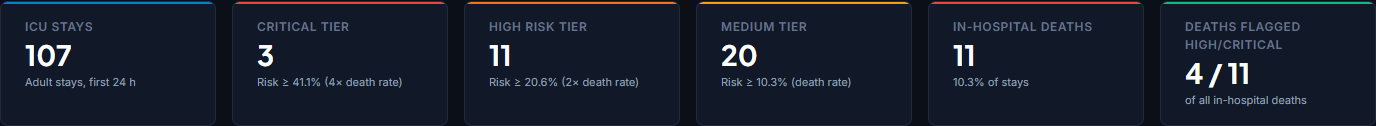
\includegraphics[width=\linewidth]{figures/screenshots/10_research_triage_kpis.png}\\[-1pt]
{\footnotesize (c) Research triage summary cards}
\caption{Research mode on the MIMIC-IV Demo (aggregate views only)}
\label{fig:ss-research}
\end{figure}

\section{Functional Results}
Each functional requirement is met by at least one passing test (Table~\ref{tab:testcases}). In the
synthetic demo every one of the 100 patients returns a tier, a score, four model votes and a non-empty
72-hour vitals series; a single-use pass grants exactly one access even under concurrent scans; research
mode refuses unsafe configuration and tampered artifacts.

\section{Performance Results}
\subsection{Server performance}
Measured server performance is reported in Chapter~\ref{ch:scal}: median prediction latency 71.9~ms for one
client, about 15 predictions/s at saturation, 268.8 simple reads/s at 16 clients, 0 errors and at most
206~MB of memory.

\subsection{Synthetic ensemble benchmark}
\label{sec:synthcaveat}
The project benchmark (\code{models_store/benchmark_report.json}, 23~October~2026) reports accuracy,
precision, recall and F1 of 1.00 on a 20-patient hold-out split and in 5-fold cross-validation, with a mean
inference latency of 24.4~ms (p95 29.5~ms). \textbf{These figures do not indicate clinical accuracy.} The
synthetic patients are generated tier by tier from tier-specific value ranges, so the tiers are nearly
separable by construction; perfect scores show only that the pipeline learns the generator.

\subsection{Research task on the MIMIC-IV Demo}
\textbf{Cohort.} Table~\ref{tab:cohort} traces the cohort (dataset v1.2.0, task v3). ``Eligible'' means
the first ICU stay of an adult admission, still alive, still in the ICU and still in hospital at the index
time (ICU admission + 24~h). The label is in-hospital death after the index time; features use only the
first 24 ICU hours. All 11 positive stays, including the 4 with a death time recorded after the discharge
time, are in the primary evaluation cohort of 107 stays; sensitivity analysis A re-scores the primary
predictions without the 4 anomalies, and B retrains without them (103 stays, 7 deaths).

\begin{table}[!htbp]
\centering
\caption{Research cohort flow (MIMIC-IV Clinical Database Demo 2.2)}
\label{tab:cohort}
\small
\begin{tabular}{@{}lr@{}}
\toprule
Step & Stays\\
\midrule
ICU stays in source & 140\\
\quad excluded: not the first ICU stay of the admission & $-12$\\
\quad excluded: died before the index time & $-1$\\
\quad excluded: left the ICU before the index time & $-20$\\
\quad excluded: ambiguous outcome fields & $0$\\
\textbf{Eligible cohort (primary evaluation)} & \textbf{107}\\
\quad positive (in-hospital death): 7 consistent + 4 flagged timestamp anomalies & 11 (10.3\,\%)\\
\quad negative & 96\\
Sensitivity cohort (anomalies removed) & 103 (7 deaths)\\
\bottomrule
\end{tabular}
\end{table}

\textbf{Baselines.} Table~\ref{tab:research} gives the pooled out-of-fold results of model set v2.0.0
(5-fold StratifiedGroupKFold by patient, seed 42; 95\,\% subject-bootstrap intervals; threshold = training
prevalence). Figure~\ref{fig:auroc} shows the AUROC intervals.

\begin{table}[!htbp]
\centering
\caption{Research baselines, primary analysis (107 stays, 11 deaths; evaluation status: limited)}
\label{tab:research}
\small
\begin{tabular}{@{}lcccc@{}}
\toprule
Model & AUROC [95\% CI] & Avg.\ precision [95\% CI] & Brier & Sens.\ / Spec.\\
\midrule
Prior-only reference & 0.46 [0.30--0.62] & 0.10 [0.05--0.17] & 0.092 & 1.00 / 0.00\\
Logistic regression & 0.74 [0.57--0.90] & 0.31 [0.14--0.62] & 0.086 & 0.73 / 0.76\\
Decision tree (smoothed) & 0.56 [0.35--0.77] & 0.15 [0.07--0.39] & 0.098 & 0.36 / 0.75\\
Random forest & 0.73 [0.53--0.91] & 0.34 [0.14--0.66] & 0.082 & 0.64 / 0.62\\
Neural network (MLP) & 0.77 [0.60--0.91] & 0.41 [0.17--0.66] & 0.087 & 0.55 / 0.85\\
\bottomrule
\end{tabular}
\end{table}

\begin{figure}[!htbp]
\centering
\begin{tikzpicture}
\begin{axis}[width=0.8\linewidth, height=50mm, ylabel={AUROC}, ymin=0.2, ymax=1.0,
  symbolic x coords={Prior,LR,DT,RF,MLP}, xtick=data, tick label style={font=\scriptsize},
  label style={font=\footnotesize}, enlarge x limits=0.15]
\addplot[only marks, mark=*, mhblue, error bars/.cd, y dir=both, y explicit]
  coordinates {(Prior,0.46) += (0,0.16) -= (0,0.16) (LR,0.74) += (0,0.16) -= (0,0.17)
               (DT,0.56) += (0,0.21) -= (0,0.21) (RF,0.73) += (0,0.18) -= (0,0.20)
               (MLP,0.77) += (0,0.14) -= (0,0.17)};
\addplot[dashed, mhred] coordinates {(Prior,0.5) (MLP,0.5)};
\end{axis}
\end{tikzpicture}
\caption{Pooled out-of-fold AUROC with 95\% subject-bootstrap intervals (Table~\ref{tab:research});
dashed line: chance (0.5)}
\label{fig:auroc}
\end{figure}

\textbf{Sensitivity analyses} (103 stays, 7 deaths). A (anomalies removed from scoring only): AUROC
LR 0.73, DT 0.52, RF 0.73, MLP 0.78. B (retrained without anomalies, folds with 1--2 deaths): LR 0.40
[0.08--0.76], DT 0.61, RF 0.71, MLP 0.39 [0.02--0.78]. \textbf{Stay-level view.} With tiers at fixed
multiples of the death rate (Medium $\ge$ 1$\times$, High $\ge$ 2$\times$, Critical $\ge$ 4$\times$
10.3\,\%), the 107 stays fall into 3 Critical, 11 High, 20 Medium and 73 Low, with 2, 2, 4 and 3 deaths
respectively; 4 of the 11 deaths were placed in High or Critical.

\section{Comparison with Existing Systems}
Compared with the systems in Table~\ref{tab:compare}, MediHaven adds patient-controlled sharing, explicit
uncertainty and fail-closed research serving, but its discrimination on real data (AUROC about 0.73--0.77
with intervals spanning roughly 0.55--0.90) is far below large-cohort models such as
\cite{rajkomar2018scalable} (0.93--0.94) and is not comparable with them, given 11 deaths and no external
validation. Bedside scores remain the only clinically validated option of those compared.

\section{Achievement of Objectives}
\begin{table}[!htbp]
\centering
\caption{Objectives and supporting evidence}
\label{tab:objectives}
\small
\begin{tabularx}{\textwidth}{@{}lYl@{}}
\toprule
Objective & Evidence & Status\\
\midrule
O1 portals and API & 44 routes; RBAC tests; Figures~\ref{fig:ss-triage}--\ref{fig:ss-portals} & achieved\\
O2 explainable ensemble & votes, rule path, KNN cases; model tests; Figure~\ref{fig:ss-triage}(b) & achieved\\
O3 secure vault and QR & scope, expiry, atomic quota, audit; TC-08 to TC-11 & achieved\\
O4 research task and evaluation & Tables~\ref{tab:cohort}--\ref{tab:research} & achieved (pipeline), performance not established\\
O5 verified research serving & hash verification, OOF reproduction; TC-14, TC-15 & achieved\\
O6 data protection & security tests; Section~\ref{sec:secdesign} & achieved for the prototype scope\\
O7 testing and measurement & 354 passing tests; Chapter~\ref{ch:scal} & achieved\\
\bottomrule
\end{tabularx}
\end{table}

\section{Discussion of Findings}
The contrast between perfect synthetic scores and modest, uncertain real-data scores is the central
finding: model quality claims depend on the data, and synthetic benchmarks validate pipelines, not
medicine. On the real cohort, the learned models beat the prior-only reference in the primary analysis,
but their intervals overlap heavily, the rankings change between analyses, and sensitivity analysis B
shows that logistic regression and the MLP collapse when only 7 deaths remain. The four timestamp anomalies
are 4 of 11 positives, so the labelling rule materially affects results. The smoothed decision tree trades
discrimination for interpretability and never outputs 0\,\% or 100\,\%.

\section{Practical Applicability}
MediHaven is suitable for teaching, demonstrations and prototyping user interfaces and data-protection
patterns. It must not be used for diagnosis, treatment or any other patient-care decision. Larger,
multi-site, credentialed data, calibration analysis, prospective evaluation and regulatory review would be
required before any clinical use could be considered.
